\documentclass{standalone}

\usepackage{tikz}
\usepackage{circuitikz}

\tikzset{block/.style = {draw, fill=white, very thick, rectangle, minimum height=1cm, minimum width=2cm},
         lblock/.style={draw,fill=white,very thick, rectangle, minimum height=3cm, minimum width=1cm},
         sum/.style= {draw, fill=white, very thick, circle, node distance=0.5cm}}

         
\begin{document}
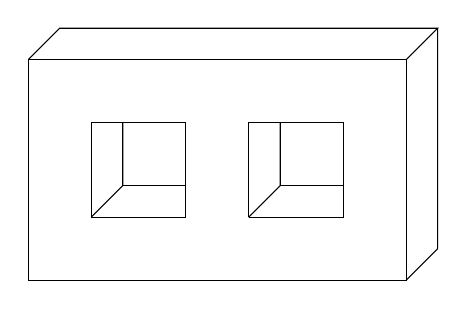
\begin{tikzpicture}[scale=0.8]
    \draw[-](0,0)--(6,0)--(6,3.5)--(0,3.5)--(0,0);
    \draw[-](1,1)--(2.5,1)--(2.5,2.5)--(1,2.5)--(1,1);
    \draw[-](3.5,1)--(5,1)--(5,2.5)--(3.5,2.5)--(3.5,1);
    \draw[-](0,3.5)--(0.5,4)--(6.5,4)--(6,3.5);
    \draw[-](6.5,4)--(6.5,0.5)--(6,0);
    \draw[-](1,1)--(1.5,1.5)--(1.5,2.5);
    \draw[-](1.5,1.5)--(2.5,1.5);
    \draw[-](3.5,1)--(4,1.5)--(4,2.5);
    \draw[-](4,1.5)--(5,1.5);
\end{tikzpicture}
\end{document}